
%%%%%%%%%%%%%%%%%%%%%%%%%%%%%%%%%%%%%%%%%%%%%%%%%%%%%%%%%%%%%%%%%%%%
\section{Organization and Management}
\label{sec:fd-daq-org}

%\metainfo{2 Pages}
At the time of writing, the \dword{daq} consortium comprises \num{30} institutions, including universities and national labs, from five countries. Since its conception, the \dword{daq} consortium has met on roughly a weekly basis, and has so far held two international workshops dedicated to advancing the  \dword{fd} \dword{daq} design. The current \dword{daq} consortium leader is Dave Newbold, U. Bristol, UK.

Several key technical and architectural decisions have been made in the last months, that have formed an agreed basis for the \dword{daq} design and implementation presented in this document.

%%%%%%%%%%%%%%%%%%%%%%%%%%%%%%%%%%%
\subsection{DAQ Consortium Organization}
\label{sec:fd-daq-org-consortium}

The DUNE \dword{daq} consortium is currently organized in the form of five active
Working Groups (WG) and WG Leaders:
\begin{itemize}
\item Architecture, WG Leaders: Giles Barr (U. Oxford) and Giovanna Lehman-Miotto (CERN);
\item Hardware, WG Leaders: David Cussans (U. Bristol) and Matthew Graham (SLAC);
\item Data selection, WG Leader: Josh Klein (U. Penn.);
\item Back-end, WG Leader: Kurt Biery (\fnal);
\item Integration and Infrastructure, WG Leader: Alec Habig
  (U. Minnesota Duluth).
\end{itemize}

During the ongoing early stages of the design, the architecture and hardware WGs have been holding additional meetings focused on aspects of the design related to architecture solutions and costing. In parallel, the \dword{daq} Simulation Task Force effort, which was in place at the time of the consortium inception, has been adopted under the data selection WG, and simulation studies have continued to inform design considerations. This working structure is expected to remain in place through at least the completion of the Technical Proposal. During the construction phase of the project we anticipate a new organization, built around major subsystem construction and commissioning responsibilities, and drawing also upon expertise build up during the \dword{protodune} projects.

%%%%%%%%%%%%%%%%%%%%%%%%%%%%%%%%%%
\subsection{Planning Assumptions}
\label{sec:fd-daq-org-assmp}

The \dword{daq} planning is based the assumption of a \dword{spmod} first, followed by a \dword{dpmod}. The schedule is sensitive to this assumption, as the \dword{daq} requirements for the two module types are quite different. Five partially overlapping phases of activity are planned (see Figure~\ref{fig:daq-schedule}):

\begin{itemize}
	\item A further period of R\&D activity, beginning at the time of writing, and culminating in a documented system design in the \dword{tdr} around July 2019;
	\item Production and testing of a full prototype \dword{daq} slice of realistic design, culminating in an Engineering Design Review;
	\item Preparation and fit out of the \dword{cuc} counting room with a minimal \dword{daq} slice, in support of the first module installation;
	\item Production and delivery of final hardware, computing, software and firmware for the first module;
	\item Production and delivery of final hardware, computing, software and firmware for the second module.
\end{itemize}

This schedule assumes beneficial occupancy of the \dword{cuc} ounting room by end of the first quarter of 2022, and the availability of facilities to support an extended large-scale integration test in 2020 (e.g., CERN or \fnal). We assume the availability of resources for installation and commissioning of final \dword{daq} hardware (e.g., surface control room and server room facilities) from around the first quarter of 2023, and the \dword{itf} from the second quarter of 2022. The majority of capital resources for \dword{daq} construction will be required from the second quarter of 2022, with a first %tranche 
portion of funds for the minimal \dword{daq} slice from the first quarter of 2021.

%%%%%%%%%%%%%%%%%%%%%%%%%%%%%%%%%%%
%\subsection{WBS and Responsibilities}
%\label{sec:fd-daq-org-wbs}

% Apparently this is no longer required? DMN

%%%%%%%%%%%%%%%%%%%%%%%%%%%%%%%%%%
\subsection{High-level Cost and Schedule}
\label{sec:fd-daq-org-cs}

The high-level \dword{daq} schedule, which is based upon the current DUNE \dword{fd} top-level schedule, is shown in Figure~\ref{fig:daq-schedule}.

\begin{dunefigure}[\dword{daq} high-level schedule]{fig:daq-schedule}
  {\dword{daq} high-level schedule}
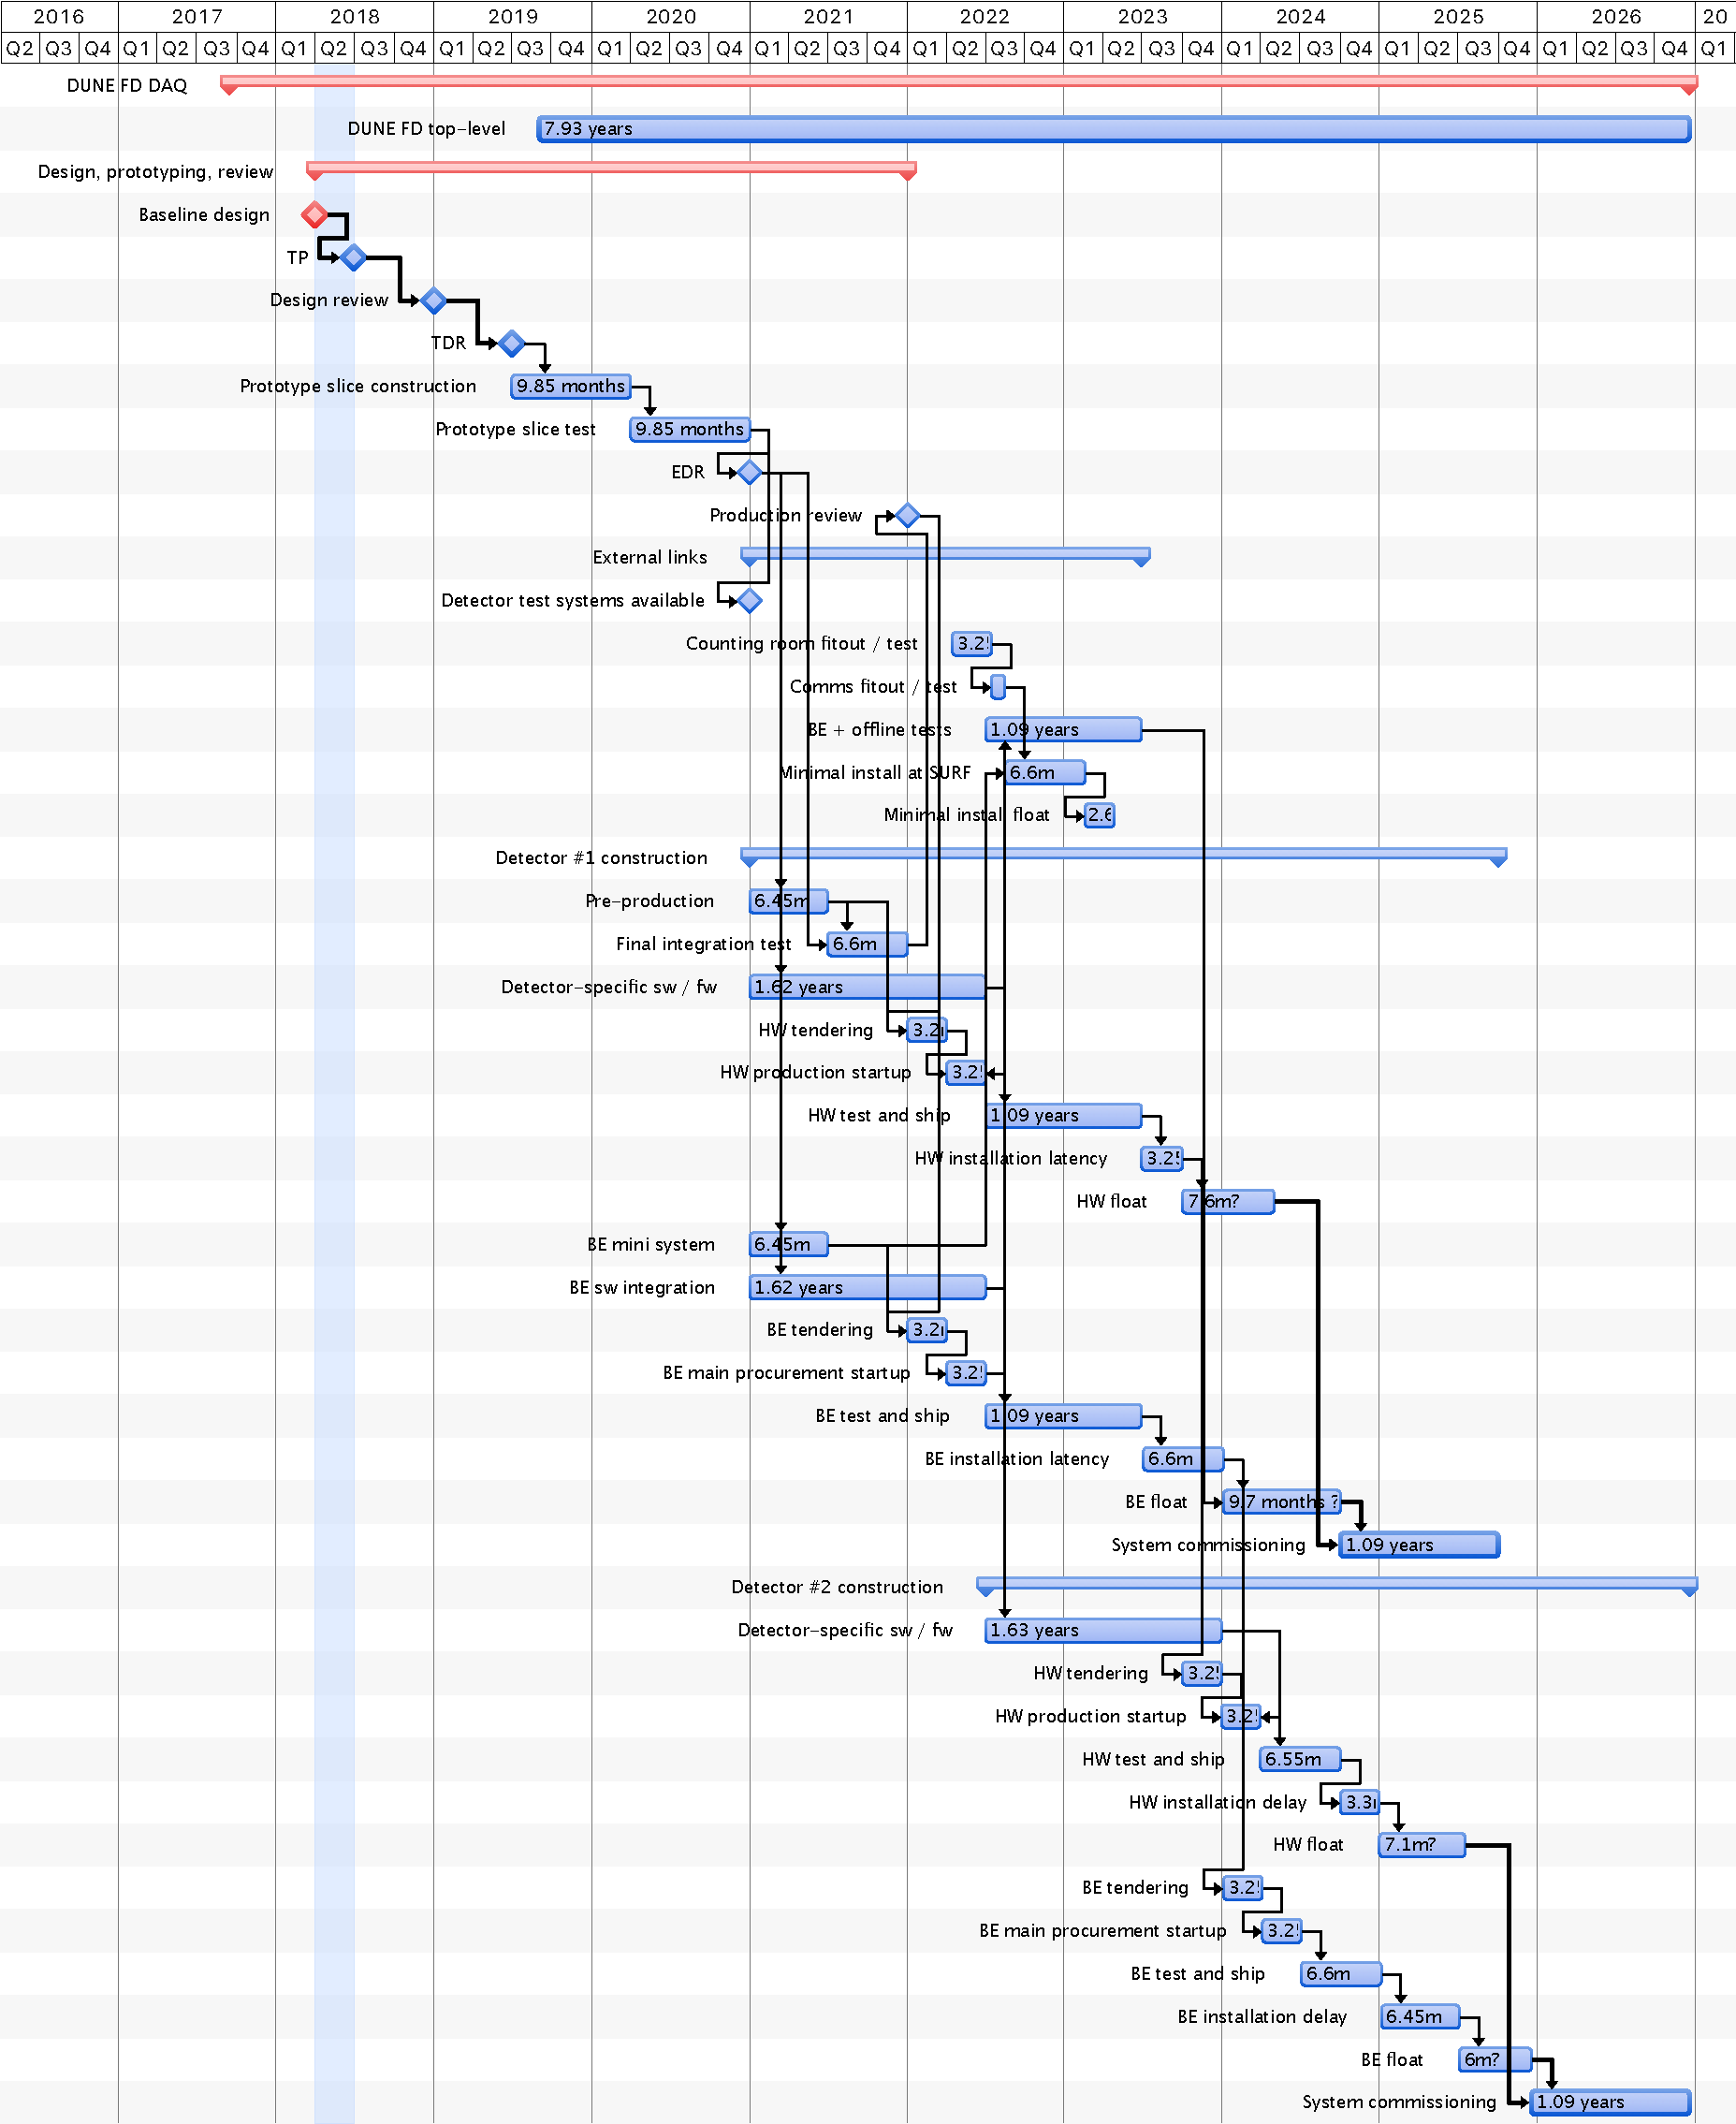
\includegraphics[width=0.8\textwidth]{DAQ-schedule.pdf}
\end{dunefigure}

%A high-level breakdown of the \dword{daq} cost for the first two detectors is summarised in Table~\ref{tab:daq-cost}.

%\begin{dunetable}[\Dword{daq} high-level cost breakdown (2017 kUSD)]{lllll}{tab:daq-cost}{\dword{daq} high-level cost breakdown} (full table in earler versions of this file 10 May )
